\documentclass[thesis.tex]{subfiles}

\begin{document}
    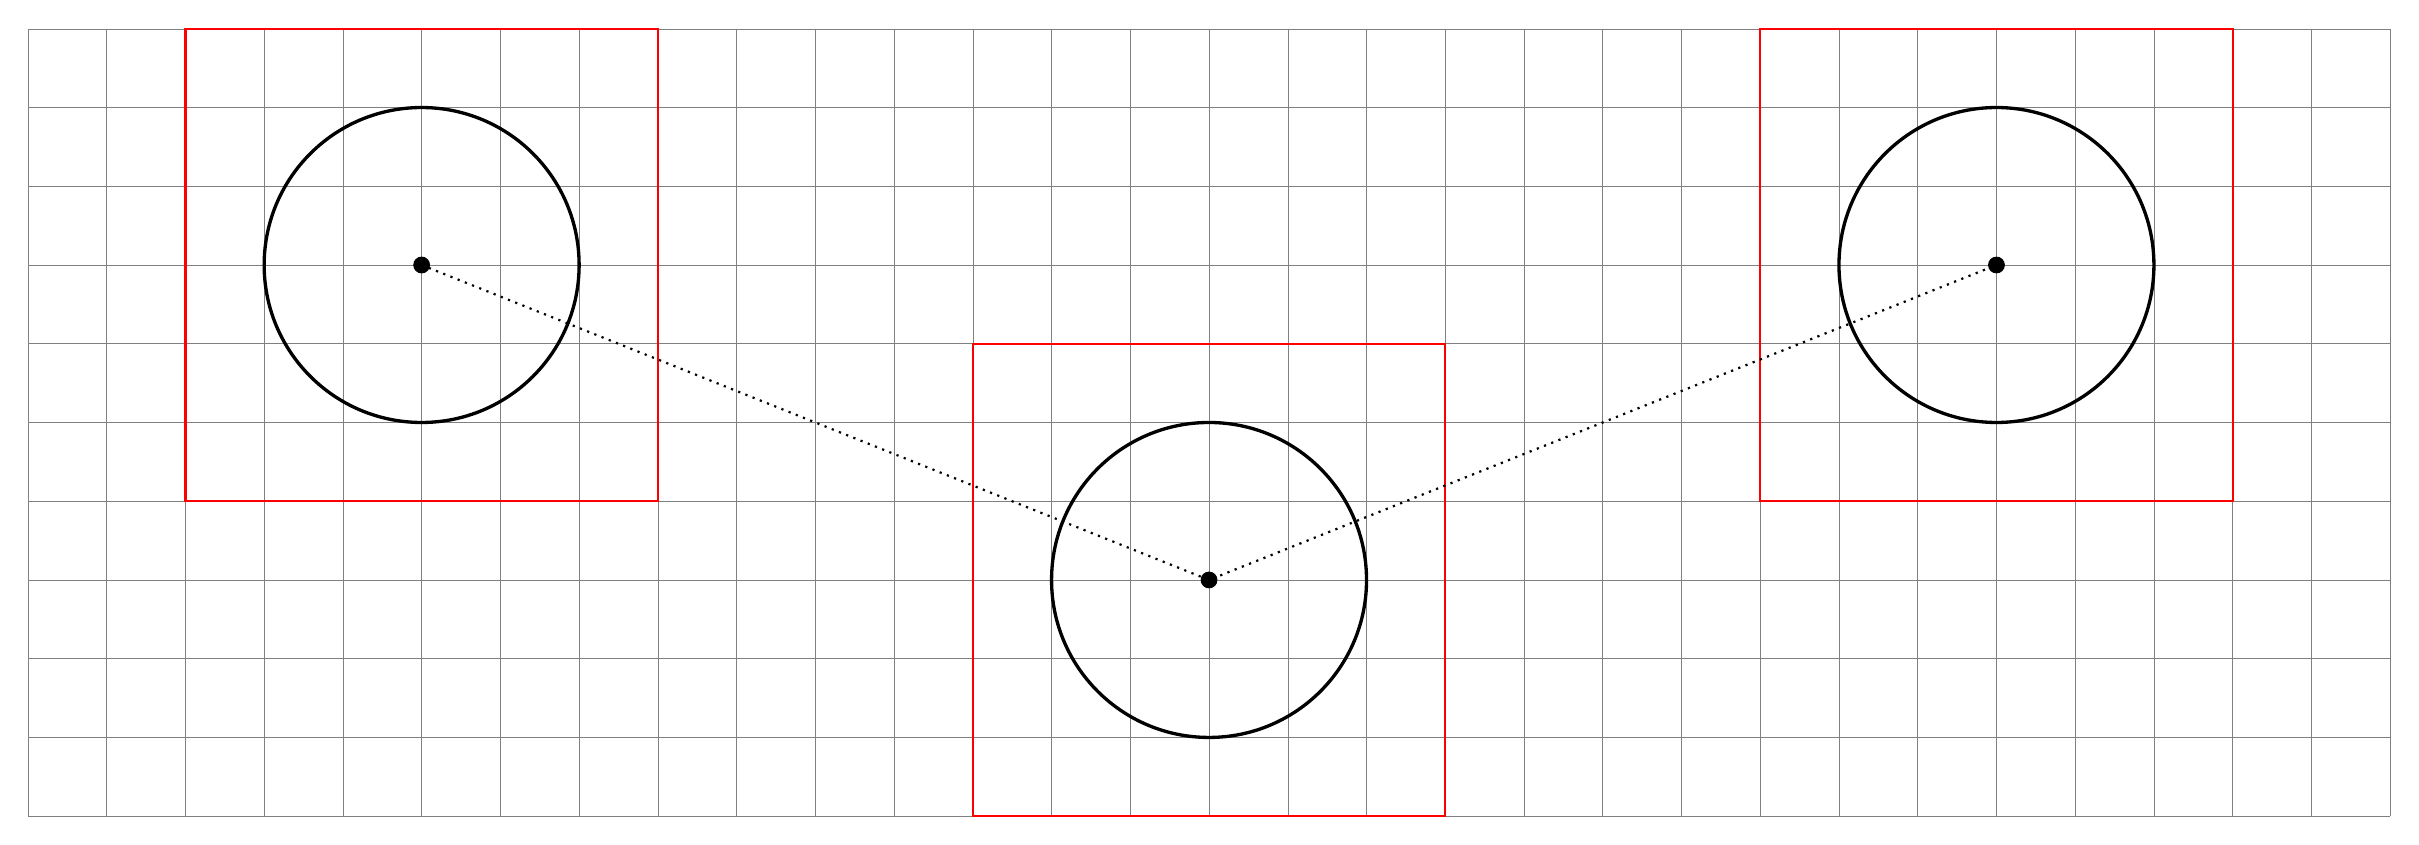
\begin{tikzpicture}
        % сетка
        \draw[step=1,gray,very thin] (-15,-5) grid (15,5);

        % первое положение
        \draw[very thick] (-10,2) circle (2);
        \draw[thick,red] (-13,-1) rectangle (-7,5);

        % второе положение
        \draw[very thick] (0,-2) circle (2);
        \draw[thick,red] (-3,-5) rectangle (3,1);

        % третье положение
        \draw[very thick] (10,2) circle (2);
        \draw[thick,red] (13,-1) rectangle (7,5);

        % траектория
        \draw[dotted,thick] (-10,2) -- (0,-2) -- (10,2);
        \node[draw,circle,inner sep=2pt,fill] at (-10,2) {};
        \node[draw,circle,inner sep=2pt,fill] at (10,2) {};
        \node[draw,circle,inner sep=2pt,fill] at (0,-2) {};
    \end{tikzpicture}
\end{document}
